\chapter{Compact Muon Solenoid}
\label{ch:CMS}

\section{The Detector}
\label{sec:cmsIntro}

The Compact Muon Solenoid (CMS) is a particle detector as part of the Large Hadron Collider (LHC) which is located near Geneva, Switzerland as part of the CERN collaboration. The CMS detector is 21.6 m long, 15 m diameter, and 14,000 tons and is used to detect many different species of particles. It is separated into layers that, from the interaction vertex outward are, the silicon tracker, Electromagnetic Calorimeter (ECAL), Hadronic Calorimeter (HCAL), superconducting solenoid, and the muon chanbers, see Fig. \ref{CMSSlice}. 

\begin{figure}
 	\centering
	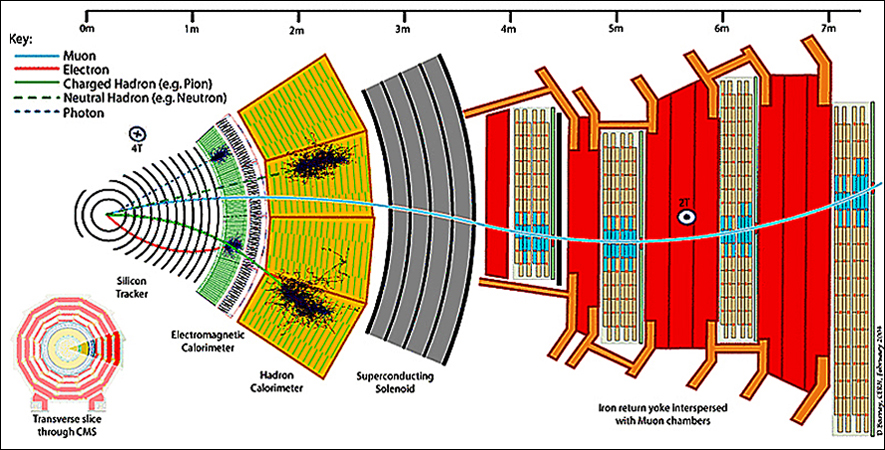
\includegraphics[width=0.75\textwidth]{cms_slice.jpg}
 	\caption{A cross-section of the CMS detector, oriented by looking down the direction of the beam pipe. }
 	\label{CMSSlice} 
\end{figure}

The CMS detector is designed to detect the decay products of most of the particles of the SM, except for neutrinos since they are weakly interacting and will almost certainly pass through the entire earth without an interaction. A defining feature of CMS is the 12.6-m long, 5.9 m inner diameter, 3.8 T superconducting solenoid. This is used to bend the trajectory of charged particles thoughout the detector, such that we can reconstruct the momentum and charge of the particles. The LHC provides a 13 TeV proton-proton beam (4.5 TeV heavy ion) beam with a bunch crossing every 25 ns (50 ns) to produce interaction at luminosities of $2.5\times10^{34} \cm^{-2}s^{-1}$. 

The coordinate system of CMS has the origin at the nominal collision point in the center of the detector. The $y$-axis points vertically upward, $x$-axis points radially inward toward the center of the LHC, and $z$-axis points along the beam directions towards the Jura mountains from LHC Point 5. The polar angle $\theta$ is measured from the $z$-axis and the azimuthal angle $\phi$ is measured in the $x-y$ plane from the $x$-axis. The pseudorapidity of a particle is defined as $\eta=-\ln\tan(\theta/2)$ where two notable values are $\eta=0$ at $\theta=\pi/2$ and $\eta=\inf$ at $\theta=0$. The transverse components of momentum, $p_T$, and energy, $E_T$, are computed using the $x$ and $y$ components of the particles. 

\subsection{Tracker}
\label{sec:Tracker}

The silicon tracker is made up of two different detectors, the silicon pixels and the silicon strip tracker. This is the inner most detector for CMS and sees the largest flux of particles during operation. This requires it to be radiation hard and operate with a fine granularity. 

\begin{figure}
 	\centering
	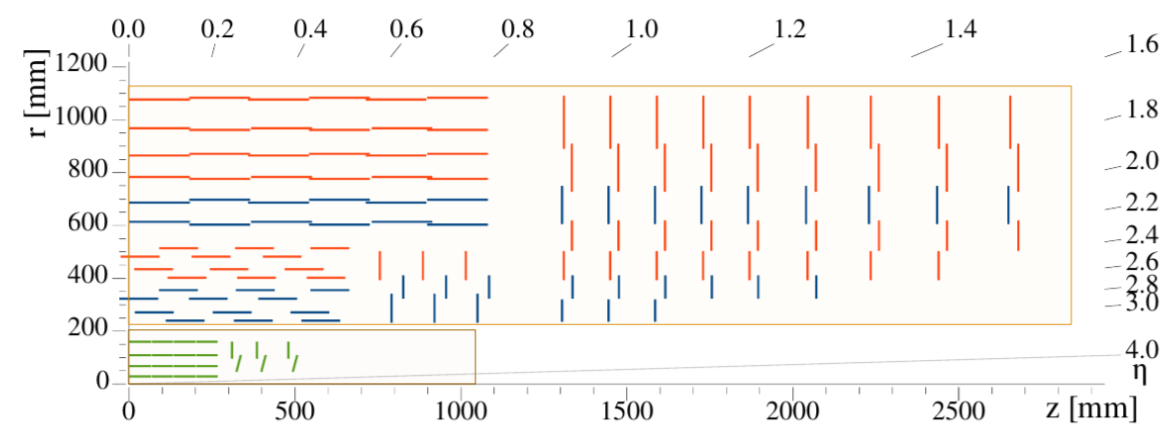
\includegraphics[width=0.75\textwidth]{Tracker_Configuration.png}
 	\caption{Geometry of the CMS Tracker, the inner most region in green is the pixel detector while the outer region in blue and red are the silicon strips.}
 	\label{CMSTracker} 
\end{figure}

\subsubsection{Pixel Detector}
\label{subsec:Pixel}

The pixel detector was recently upgraded during the winter of 2016/2017. It is approximately 1 m long with four barrel layers ranging from 3.0, 6.8, 10.2, and 16.0 \cm{} and three endcap disks, see fig. \ref{CMSTracker}. Since it is the closest detector to the interaction vertex it therefore has the highest particle flux at $10^7/\cm^2/s$ at $r\equiv10$ cm. The resolution is $9.4$ \mum{} in $r-\phi$ and $20-45$ \mum{} in $z$.

\begin{figure}
 	\centering
	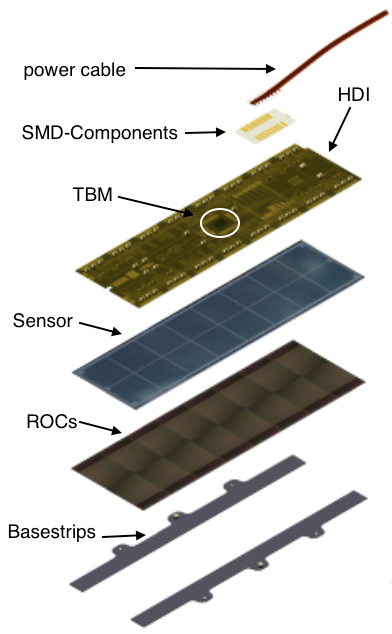
\includegraphics[width=0.5\textwidth]{Pixel_Module.png}
 	\caption{Components of the pixel modules. Made up of a silicon layer, a grid of 8 ROCs which are attached via bump bonds. This is all controlled with a TBM connection to read out data.}
 	\label{PixelModule} 
\end{figure}

The pixel detector contains 1184 modules in the barrel pixels (BPIX) and 672 modules in the forward pixels (FPIX). The number of individual pixels is 79 (45) million in the BPIX (FPIX) regions, respectively, with a pixel size of $100\times150 \text{ }\mum^2$. A pixel module contains two layers, a silicon layer that is bump bonded to 16 Readout Chips (ROCs) which form a module of 66560 pixels, see fig. \ref{PixelModule}. Each unit is controlled with one or more Token Bit Managers (TBMs) which controls the readout of the digital signal from the pixels to the Front-end Driver (FED). For BPIX Layers 3,4 and all of FPIX there is 1 TBM per module. BPIX layer 2 has 2 TBMs with each one controlling 8 ROCs, while BPIX layer 1 has 4 TBMs with each one controlling 4 ROCs. The information from each module is split into two channels with each containing 8 ROCs. These are encoded together by the TBM before being sent to the FED.

The silicon pixel system is set up as a reverse p-n junction, where the pixels are in the n-type region. As a charged particle travels through the silicon it creates electron-hole pairs. A voltage difference is applied to the silicon such that the electrons will deposit onto the pixels. Since the detector is inside of the magnetic field, a lorentz drift will cause the electrons to reach more than one pixel and increase the resolution. As the pixel system continues to be irradiated with large quantities of particles the voltage in the silicon decreases. This will lead to less charge sharing between the pixels and a decrease in resolution of particle locations. 

\begin{figure}
 	\centering
	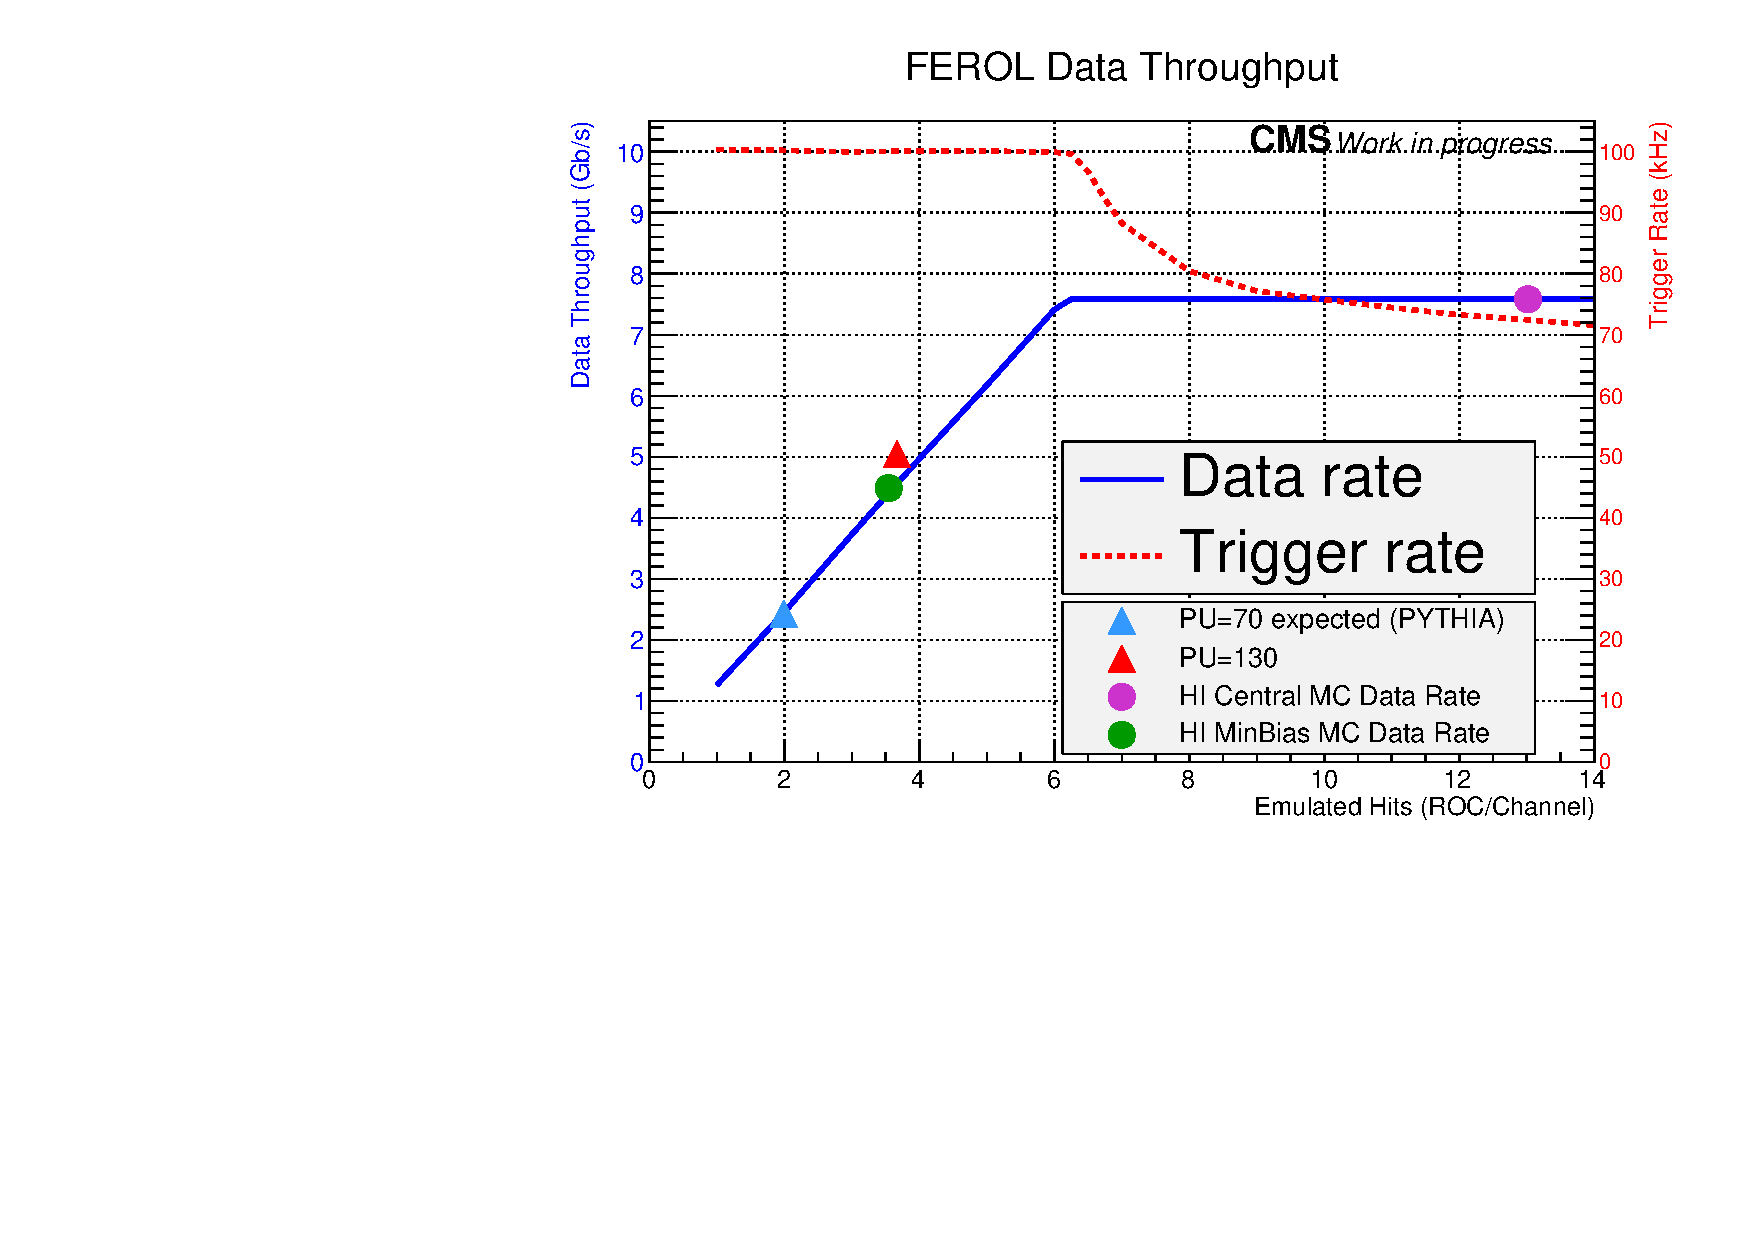
\includegraphics[width=0.75\textwidth]{FEROL_Data_Throughput_Thesis.pdf}
 	\caption{Measuring the throughput of the FED with the emulated and simulated events provided by the FED Tester. The Data rate is shown as the solid blue line with the corresponding trigger rate as the dotted red line. The simulated event sizes are shown as their equivalent emulated hits/ROC/channel on the data line.}
 	\label{FEDThroughput} 
\end{figure}

The data, from the pixels, is sent via optical fiber to the FED where it decodes and processes the information. The FED is responsible for identifying the relevant data, determining possible error states, and packaging the information to be sent to the central Data Acquisition (cDAQ) of CMS. Each of the 108 FEDs, for the pixels, receives 24 independent fibers from the detector. Each of these fibers contains 2 channels from the pixel module. Through robust testing with the FED Tester [Cite here], we have confirmed that the FED is able to attain a maximum data throughput of approximately 7.5 Gbps, see fig. \ref{FEDThroughput}. 

\subsubsection{Silicon Strips}
\label{subsec:Strips}

The silicon strips have a 200 m$^2$ active region with 15148 modules that are distributed in 10 barrel layers and $9+3$ endcap disks.
This has a cell size ranging from $10 \cm \times80$ \mum{} to $25 \cm \times 180$ \mum{} since the particle flux decreases further away from the vertex, [MAYBE ANOTHER FIGURE]. It has a resolution of $23-24$ \mum{} in $r-\phi$ and $23$ \mum{} in $z$ for the microstrip tracker

How is it different from the pixels?

\subsection{Electromagnetic Calorimeter}
\label{sec:ECAL}

The ECAL is a homogeneous calorimeter made out of 61200 lead tungstate $(\text{PbWO}_4)$ crystals in the barrel and 7324 crystals in each endcap. The barrel region has an inner radius of 129 cm and covers a pseudorapidity range of $0<|\eta|<1.479$. The encaps are 314 cm from the interaction point and cover a range $1.479<|\eta|<3.0$ in pseudorapidity. Lead tungstate was chosen for teh crystals since it has a short radiation length, $X_0=0.89\cm$, fast with 80\% of the light being emitted within 25 ns, and it's radiation hard. Each crystal in the barrel has a cross-section of $\approx22\times22 \text{mm}^2$ and length of 230 mm, while the endcap crystals are $28.6\times28.6 \text{mm}^2$ and length of 220 mm corresponding to $25.8X_0$ and $24.7X_0$, respectively. An ECAL uses electromagnetic showers to detect charged particles or photons that interact electromagnetically. Electrons traveling through the material will radiate a photon via bremsstrahlung. A photon will pair produce two electrons. Combining these two processes leads to electromagnetic showers as the particles travel through the detector. The process will continue until a critical energy is reached such that an electron cannot radiate any further and will then lose energy via collisions. The resulting light is recorded by silicon avalanche photodiode (vaccuum phototriodes) in the barrel (endcap). 

\subsection{Hadronic Calorimeter}
\label{sec:HCAL}

The HCAL is a hermetic calorimeter consisting of alternating layers of brass as the absorber material and a scintillator. Brass is chosen since it is non-magnetic and has a relatively short interaction length. In the scintillator, a portion of the energy from the hadron in converted into visible light which is then measured by a hybrid photodiode tube to measure the energy. The barrel part of the HCAL consists of 2304 towers that are segmented into $\Delta\eta\times\Delta\phi=0.087\times0.087$ pieces that cover a region $0<|\eta|<1.4$ in pseudorapidity. The encap region consists of 2304 towers with varying segmentation sizes and a coverage of $1.3<|\eta|<3.0$. 

There are two additional parts of the HCAL to allow for maximum coverage of the detector volume. There is a outer hadron detector that is located outside the superconducting solenoid, which covers a slightly smaller pseudorapidity range as the barrel region. They serve as a tail catcher for hadron showers that penetrate all the way through the inner HCAL and solenoid. A forward hadron calorimeter, located 11.2 m from the interaction point covering a pseudorapidity $3.0<\eta<5.0$, made out of steel/quartz fiber is specifically designed for the columnated Cerenkov light in this region. 

\subsection{Superconducting solenoid}
\label{sec:Solenoid}

Containing all of this is the superconducting solenoid which is 12.6 m long and a 5.9 m radius. The field strength is 3.8 T which has a stored energy of approximately 2.7 GJ. The magnet is designed such that a muon with momentum, $p=1$ TeV, will have a momentum resolution of $\Delta p/p\approx10\%$. The solenoid is a high-purity aluminium-stabilized conductor, which is a similar material used in other large solenoids. 

\subsection{Muon Chambers}
\label{sec:muCham}

The muon system has three main detection systems that are use to identify a muon candidate. In the barrel region, drift tube (DT) chambers are used since the neutron background, muon rate, and magnetic field are all small. In the endcaps, cathode strip chambers (CSCs) are used since the relative values stated before are much larger. Included throughout the whole system are resistive plate chambers (RPC). 

\begin{figure}
 	\centering
	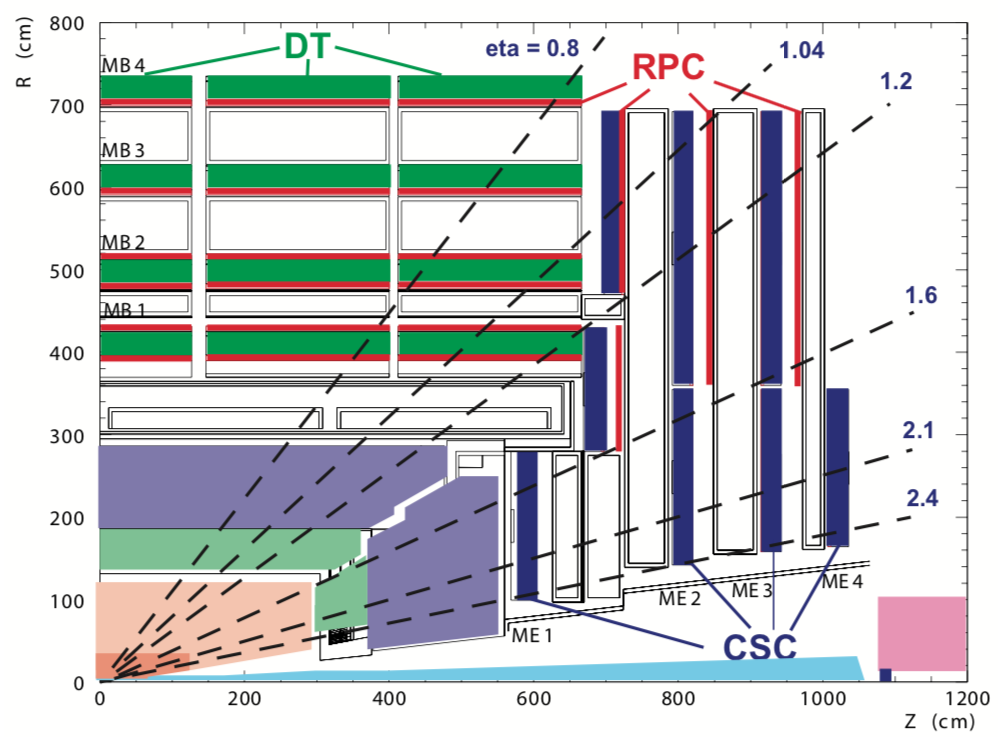
\includegraphics[width=0.75\textwidth]{MuonChambers.png}
 	\caption{A quarter cross-section of the three detection systems for CMS. }
 	\label{MuonChambers} 
\end{figure}

The DT consists on 250 chambers in 4 barrel layers at a radii of 4.0, 4.9, 5.9, and 7.0 m from the beam axis. A DT chamber is an array of anode wires in a gaseous medium where the walls are cathodes. A muon passing through the gas will ionize some atoms which are then forced towards the anode wires by an electric field. The drift time of the electrons can then be calculated to within a couple of ns such that a good spatial resolution is achieved. The maximum designed drift length is 2.0 cm. Each station of the DT will give muon vector for each candidate with a $\phi$ precision of 100 \mum{} in postion and 1 mrad in direction. 

The CSC system uses the same concept as the DT system, but also includes a measurement of the ions that follow the electric field to the cathode strips. In this system the anode wires and the cathode strips are perpendicular so the collected charge on both provide a accurate position measurement. 

The RPC system contains two parallel plates, anode and cathode, the charge is measured by external metallic strips that can quickly measure the momentum of a muon and decide if the event is worth triggering.

